% Copyright (C) 2019 Cui Jialiang ( SESS, PKU ). All rights reserved.

%                       _oo0oo_
%                      o8888888o
%                      88" . "88
%                      (| -_- |)
%                      0\  =  /0
%                    ___/`---'\___
%                  .' \\|     |// '.
%                 / \\|||  :  |||// \
%                / _||||| -:- |||||- \
%               |   | \\\  -  /// |   |
%               | \_|  ''\---/''  |_/ |
%               \  .-\__  '-'  ___/-. /
%             ___'. .'  /--.--\  `. .'___
%          ."" '<  `.___\_<|>_/___.' >' "".
%         | | :  `- \`.;`\ _ /`;.`/ - ` : | |
%         \  \ `_.   \_ __\ /__ _/   .-` /  /
%     =====`-.____`.___ \_____/___.-`___.-'=====
%                       `=---='
%
%
%     ~~~~~~~~~~~~~~~~~~~~~~~~~~~~~~~~~~~~~~~~~~~
%
%               佛祖保佑         顺利毕业

% \documentclass[UTF8,openany]{pkuthss}
\documentclass[UTF8,openany]{tex/pkuthss_local} % 使用本地模板(pkuthss 1.8.0)

% 使用 biblatex 排版参考文献,并规定其格式(详见 biblatex-caspervector 的文档)。
% 这里按照英文文献在前,中文文献在后排序(“sorting = ecnty”);
% 若需按照中文文献在前,英文文献在后排序,请设置“sorting = centy”;
% 若需按照引用顺序排序,请设置“sorting = none”。
% 若需在排序中实现更复杂的需求,请参考 biblatex-caspervector 的文档。
\usepackage[backend = biber, style = caspervector, utf8, sorting = none]{biblatex}

% 按学校要求设定参考文献列表中的条目之内及之间的距离。
\setlength{\bibitemsep}{3bp}
% 对于 linespread 值的计算过程有兴趣的同学可以参考 pkuthss.cls。
\renewcommand*{\bibfont}{\zihao{5}\linespread{1.27}\selectfont}

% 设定文档的基本信息。
\pkuthssinfo{
	cthesisname = {硕士研究生学位论文}, ethesisname = {Masters Thesis},
	ctitle = {基于像素级处理技术的视频目标跟踪算法研究}, etitle = {A Research of Video Object Tracking Altorithm based on Pixel-wise Processing Technology},
	cauthor = {崔家梁},
	eauthor = {Cui Jialiang},
	studentid = {1601210300},
	date = {2019年5月},
	school = {地球与空间科学学院},
	cmajor = {摄影测量与遥感}, emajor = {Photogrammetry and Remote Sensing},
	direction = {数字摄影测量与遥感数字成像},
	cmentor = {赵红颖\ 副教授}, ementor = {Prof.\ Zhao Hongying},
	ckeywords = {数字视频处理,目标跟踪,像素级别}, ekeywords = {Digital video processing, Object tracking, Pixel-level}
}
% 载入参考文献数据库(注意不要省略“.bib”)。
\addbibresource{thesis.bib}

\usepackage{color, rotating}

\begin{document}
	% 以下为正文之前的部分,默认不进行章节编号。
	\frontmatter
	% 此后到下一 \pagestyle 命令之前不排版页眉或页脚。
	\pagestyle{empty}
	% 自动生成封面。
	\maketitle
	% 版权声明。封面要求单面打印,故需新开右页。
	\cleardoublepage
	% Copyright (c) 2008-2009 solvethis
% Copyright (c) 2010-2017 Casper Ti. Vector
% All rights reserved.
%
% Redistribution and use in source and binary forms, with or without
% modification, are permitted provided that the following conditions are
% met:
%
% * Redistributions of source code must retain the above copyright notice,
%   this list of conditions and the following disclaimer.
% * Redistributions in binary form must reproduce the above copyright
%   notice, this list of conditions and the following disclaimer in the
%   documentation and/or other materials provided with the distribution.
% * Neither the name of Peking University nor the names of its contributors
%   may be used to endorse or promote products derived from this software
%   without specific prior written permission.
%
% THIS SOFTWARE IS PROVIDED BY THE COPYRIGHT HOLDERS AND CONTRIBUTORS "AS
% IS" AND ANY EXPRESS OR IMPLIED WARRANTIES, INCLUDING, BUT NOT LIMITED TO,
% THE IMPLIED WARRANTIES OF MERCHANTABILITY AND FITNESS FOR A PARTICULAR
% PURPOSE ARE DISCLAIMED. IN NO EVENT SHALL THE COPYRIGHT HOLDER OR
% CONTRIBUTORS BE LIABLE FOR ANY DIRECT, INDIRECT, INCIDENTAL, SPECIAL,
% EXEMPLARY, OR CONSEQUENTIAL DAMAGES (INCLUDING, BUT NOT LIMITED TO,
% PROCUREMENT OF SUBSTITUTE GOODS OR SERVICES; LOSS OF USE, DATA, OR
% PROFITS; OR BUSINESS INTERRUPTION) HOWEVER CAUSED AND ON ANY THEORY OF
% LIABILITY, WHETHER IN CONTRACT, STRICT LIABILITY, OR TORT (INCLUDING
% NEGLIGENCE OR OTHERWISE) ARISING IN ANY WAY OUT OF THE USE OF THIS
% SOFTWARE, EVEN IF ADVISED OF THE POSSIBILITY OF SUCH DAMAGE.

% 此处不用 \specialchap,因为学校要求目录不包括其自己及其之前的内容。
\chapter*{版权声明}
% 综合学校的书面要求及 Word 模版来看,版权声明页不需加页眉、页脚。
\thispagestyle{empty}

任何收存和保管本论文各种版本的单位和个人,
未经本论文作者同意,不得将本论文转借他人,
亦不得随意复制、抄录、拍照或以任何方式传播。
否则一旦引起有碍作者著作权之问题,将可能承担法律责任。

% 若需排版二维码,请将二维码图片重命名为“barcode”,
% 转为合适的图片格式,并放在当前目录下,然后去掉下面 2 行的注释。
%\vfill\noindent
%
\includegraphics[height = 5em]{barcode}

% vim:ts=4:sw=4


	% 此后到下一 \pagestyle 命令之前正常排版页眉和页脚。
	\cleardoublepage
	\pagestyle{plain}
	% 重置页码计数器,用大写罗马数字排版此部分页码。
	\setcounter{page}{0}
	\pagenumbering{Roman}
	% 中英文摘要。
	% Copyright (C) 2019 Cui Jialiang ( SESS, PKU ). All rights reserved.

\begin{cabstract}
	目前,深度学习和视频目标跟踪是数字图像处理领域热门的研究方向,在遥感观测应用中有重要的研究意义。而以深度学习为核心方法的各种视频目标跟踪算法,算法结构复杂,计算效率低,需要改进,同时像素级视频目标跟踪算法作为一种新方法也需要进一步深入研究。因此,论文提出了改进的基于深度学习的像素级视频目标跟踪算法,具有重要的理论研究意义和应用价值。
	\par
	论文研究了像素级视频目标跟踪问题和相关研究的现状。论述并分析了现有的视频跟踪算法和深度学习技术。基于深度学习技术,参考加密-解码结构的图像分割算法与近期少量的像素级目标跟踪算法研究,论文提出了一种结构简单对称的像素级视频目标跟踪算法,将循环神经网络结构加入了各个尺度的卷积层中,在多个尺度上进行跟踪处理。该算法在足够的计算资源下可以实现实时像素级目标跟踪计算。
	\par
	论文详细论述了所提出算法的结构。为了验证该算法的有效性,论文设计了实验与评估体系。实验结果表明,论文提出的算法有较好的像素级视频目标跟踪效果。
\end{cabstract}

\begin{eabstract}
	Video object tracking is becoming a popular research field in digital image processing. Pixel-wise video object tracking playes an important application role, but research on it appeares rarely. Deep learning has become major thought of video and image processing. Video object tracking algorithms based on deep learning usually have difficult archtectures. 
	\par
	We conclude the related research of pixel-wise video object tracking, and analysed the existed problems. Then we proposed an pixel-wise video object tracking algorithm based on deep learning technology and encode-decode like image segmentation algorithm which can play a real time processing with sufficient compute resources. The algorithm uses recurrent neural network in each scale of convolutional neural network to produce a multi-scale tracking effect.
	\par
	We descripted the algorithm in details, including its technology background and reason of design. And we proposed an experiment to verify it.By the result of the experiment, it shows strong ability on video object tracking.
\end{eabstract}

% vim:ts=4:sw=4

	% 自动生成目录。
	\setcounter{tocdepth}{3} % 设置目录级数
	\tableofcontents

	% 以下为正文部分,默认要进行章节编号。
	\mainmatter
	% Copyright (C) 2019 Cui Jialiang ( SESS, PKU )。 All rights reserved。

\chapter{绪论}
本章将介绍本研究\footnote{指基于像素级处理技术的视频目标跟踪算法研究,后文将继续称之为本研究}的研究背景与研究意义。

\section{研究背景}
本节将介绍视频目标跟踪,像素级处理,深度学习等基础概念。这将为后文详细介绍本研究打下基础。

\subsection{视频目标跟踪问题}
视频(Video;影片[港澳台])可以看作一个图像序列\footnote{本研究中不考虑视频中的音频信息},由连续曝光获取的图像组成。很多情况下,尤其是利用摄像机在对特定的对象进行观察时,视频中将会长期存在一个或多个需要关注的目标。典型的会出现在视频中的目标可以是人物,车辆,动物等。如何使用计算机从视频中高效地持续锁定这些目标是计算机视觉,遥感等研究者十分关注的问题。
\par
在无人机应用场景中,视频目标跟踪是一项很重要的应用。广义上的无人机目标跟踪包括无人机对目标进行识别,定位,追踪的整套过程。本研究关注的视频目标跟踪主要指这其中利用计算机对视频中的目标进行持续的定位这一过程。
\par
受限于目前小型计算机和嵌入式平台有限的计算能力,我们不能随意增大视频跟踪算法的规模,因为在大多数情况下不能实时进行目标跟踪的方法是没有意义的。因此视频目标跟踪算法必须要节约计算资源。因而算法的设计就显得格外重要。

\subsection{像素级图像与视频处理技术}
在遥感应用中,对地物的识别需要用到各种各样的图像和视频处理技术。先以图像处理为例,一种图像处理技术的输入通常都是图像,而输出可以有很多种。在算法层面,图像处理技术得到的结过通常是标签+位置。如在遥感地物分类的任务中,算法给出的结果是每个像元的类型归属;在无人机目标跟踪任务中,算法给出的结果是目标所在的大致位置。根据输出形式的不同,常见的图像和视频处理算法的结果主要有像素级,矩形级和图像级等表现形式。
\par
像素级(Pixel-wise)的处理算法输出结果是一副和原图像尺寸大小几乎相同的图像
\footnote{在某些特殊情况下,如处理过程中使用了某种滤波算法,处理结果会丢失一些图像边缘信息,可能比原图小一些}
;矩形级(Box-wise)的图像处理算法的输出结果通常是一个目标的外包矩形(Bounding Box)和目标所属的标签,不需要精确到每个像素,只关注兴趣目标的大致位置和大致形状即可
;图像级的图像处理算法指给整张图片贴上一些标签,如图像中有没有某个目标,有哪些类型的目标等等。
\par
像素级的图像处理算法的典型应用有图像分割(Image Segmentation),遥感地物分类(图像像素级分类)等。这些应用需要关注到图像的每一个像素,使每一个像素有唯一的明确的归属,并且这些应用十分关心图像中不同类型的区域的边界线。
\par
矩形级的图像处理算法的典型应用有图像目标检测(Image Object Detection)和矩形框视频目标跟踪等。由于最终的需求只关心目标的大致形状和位置,矩形级的图像处理算法设计上通常会放弃一些像素级的特征。
\par
图像级的图像处理算法则处理更大尺度的问题。通常只需宏观上得到正确的结果即可。如图像分类\supercite{imagenet_cvpr09},就是图像级的处理。近年来备受关注的视频字幕生成\supercite{aswin2019nlp}也是这样的应用。

\par
从生成的结果看,像素级处理技术得到的结果自由度最高,其次是矩形级,而图像级只需要得到一个标签,结果自由度最低(这里只考虑生成目标标签的算法,不包括字幕生成等)。

\subsubsection{像素级视频目标跟踪问题}
目前主流的视频目标跟踪研究都是在试图解决矩形框视频目标跟踪问题,且大多数算法设计之初就是为产生矩形级结果而设计,其中几乎没有提取像素级结果的过程。也有少数像素级跟踪算法,但没有用到最新的图像处理技术。
\par
区别于现在大多数矩形级的目标跟踪算法,本文提出的像素级目标跟踪算法将直接以得到精确的像素级的跟踪结果为目标。

\subsection{深度学习技术}
深度学习是目前火热的一项计算机技术。近年来由于深度学习学派的强势,传统的图像处理算法几乎都被深度学习替代。深度学习由于其简单的仿生结构,严谨的概率论理论基础,十分容易被陷入困境的图像视频研究者接受。
\par
深度学习中的卷积神经网络十分利于图像处理,而循环神经网络十分利于时间序列分析。本研究结合了这两点,用深度学习实现了视频处理。

\newpage
\section{研究意义}
本文研究像素级目标跟踪算法具有重大的意义。本节后文将详细介绍。
\subsection{选题来源}
在我做本科毕业设计\supercite{benchme}时,就曾考虑到无人机影像处理过程中缺乏能将兴趣目标精确提取出的方法。随着研究的深入,我发现近年来在计算机视觉的研究中常用的深度学习方法十分适合解决这个问题。然而将计算机视觉中的视频跟踪的方法主要针对自动驾驶等领域,将其直接运用于无人机航拍的视频效果并不好,并且大多数方法无法达到遥感所需要的像素级别处理的需求。因此我选择了研究针对视频中目标的像素级别跟踪这一问题。
\par
在工业界推动下计算机学者们已经研究出很多成熟的像素级图像处理算法,将其目标稍加改动,即可运用在视频,从而有希望在无人机影像处理中得到较好的效果。

\subsection{研究视频跟踪的重要性}
视频是无人机遥感应用的重要信息载体。在需要持续观察并关注的遥感应用场景中,可见光视频由于其较容易获取,其结果较容易直接被人理解,一直是遥感应用中最常用也是最直观的信息载体。
\par
随着各种无人机实验的展开,无人机在国土安全,灾害监测,生态环境等领域都将派上巨大用场。而在这些场景下视频目标跟踪都是重要的应用。如国土安全中跟踪抓捕逃犯,灾害中寻找需要营救的人员,生态中关注动植物等。目前的目标跟踪算法并不能满足这些应用。
\par
由于现阶段的无人机平台已经实现轻量化,用无人机来跟踪目标是理所当然的最佳选择。然而现在用于无人机的跟踪算法依然不够强劲。现有的跟踪算法大多只能在大体积,高功率的服务器上运行,并且想获得好的跟踪效果就要加大模型,增加功耗。因此还无法向无人机平台迁移。算法的创新研究依然任重道远。

\subsection{现阶段视频跟踪算法缺陷}
现有的跟踪算法为了达到跟踪效果,通常需要结合多种跟踪方法,并进行结果的融合。从算法层面看,这样的结构既不高校,也不美观。实际上,由于根本理论方法的缺乏,一些算法不得不设计得越来越复杂。这种情况下需要新的思路来打破局面。
\par
视频目标跟踪算法由于要面临视频时间和空间纬度的大量数据,单位时间接受到的信息量极大。目前的多种跟踪方式均无法准确的从这些信息中提取到最少量的有效信息。算法的质的提升任然需要理论的创新。本文研究的主要是像素级别的目标跟踪。通过研究像素级别的目标跟踪,或许能获得对现有的外包矩形目标跟踪算法理论上的帮助,让产生式跟踪模型(第2章中将会介绍)重新受到重视。

% vim:ts=4:sw=4
	% Copyright (C) 2019 Cui Jialiang ( SESS, PKU ). All rights reserved.

\section{研究现状}
本节将介绍像素级视频影像跟踪算法及其相关算法的研究现状,为下一章介绍本研究的理论创新铺垫基础。
\par
需要提前指出的是,本文所提出方法将是像素级别的处理技术在视频目标跟踪问题上的一个应用,并不是现在狭义上定义的视频目标跟踪算法.但其中很多思想借鉴了现在的视频目标跟踪算法.因此在研究现状部分我们依然会着重分析视频目标跟踪算法,同时将介绍像素级别处理技术与深度学习思想.

\subsection{视频跟踪算法}
这里介绍的视频目标跟踪算法均是矩形级算法.视频目标跟踪是目前视频处理的一个很热门的研究方向.
\par
视频跟踪算法主要分为产生式模型和判别式模型.
\par
产生式模型指基于当前时刻及前一段时间的目标状态,结合新加入的帧的视频内容,直接根据概率模型产生一个新的跟踪目标.在计算能力极差的八九十年代,许多早期的模型
\supercite{schalkoff1982model}
都是产生式模型.直到20世纪初,产生式模型依然是主流.基于Kalman滤波的许多模型
\supercite{kim2002fast, weng2006video, comaniciu2003kernel}
都为推动跟踪效果做出过贡献.
\par
然而在现在(2018年),判别式模型已经完全占据了视频目标跟踪的主流.2012年Hinton提出AlexNet 
\supercite{krizhevsky2012imagenet} 
后,深度学习这一划时代的思想迅速站上了图像处理界的主流.由于卷积神经网络
\supercite{krizhevsky2012imagenet} 
(Convolution neural network)在图像处理的普适性,在
图像分类\supercite{krizhevsky2012imagenet, witten2016data, he2016deep},
图像分割\supercite{long2015fully}和
目标检测\supercite{ren2015faster, redmon2016you}
等方面均赢得了学界的认可,迅速与传统方法结合,成为这些研究方向必不可少的重要方法.在视频跟踪问题上,深度学习方法同样有较好的表现.经过几年发展,脱颖而出的基于深度学习的视频目标跟踪算法主要都是判别式模型.判别式模型指分两步完成跟踪的一种模型,第一步是利用提取特征的方法,将新帧作为一个图像做特征提取运算;第二步是结合提取出的特征和之前的跟踪结果,在提取出的特征中选择要跟踪的目标.具有代表性的有2016年的MDNet \supercite{nam2016mdnet}算法.该算法的主要思想是利用一个预先训练好的深度神经网络将送入的新帧作为图像提取特征,再形成多个次级网络进行目标跟踪.还有一些基于检测的目标跟踪,如ROLO\supercite{ning2016spatially}算法,先利用目标检测技术检测出很多目标,再从这些目标中选择一个和正在跟踪的目标比较像的目标作为跟踪结果.
\par
如前文所说,由于当今计算能力的爆发,由于能很快得到大量的目标检测结果,判别式模型大行其道.但判别式模型从思想上是目标检测的产物,其执行过程中将花费大量的时间去生成根本不是被跟踪目标的其他目标.本文将提出的是一种生成式模型,试图重新从目标跟踪的本质任务出发.

\subsection{像素级图像处理算法}
区别于典型的图像分类与目标外包框检测问题,像素级别(Pixel-wise)的图像处理需要获得一个覆盖全图的,精确到目标轮廓信息的结果.现在最常见的像素级别应用是图像分割.在图像分割领域,以早期的分水岭算法
\supercite{olsen1997multi}
为代表的传统阵营
\footnote{这里的传统阵营指用非神经网络方法的算法的处理方式}
已经有一系列研究.虽然分水岭算法有许多改进
\supercite{grau2004improved}
,但只能在大尺度图像上表现较好.对复杂情况下的分割效果依然不够智能.在深度学习技术出现后,深度学习很快就被运用于分割领域.最成功的典型是由U-Net
\supercite{ronneberger2015u}
开创的降级-升级模型.与之类似的还有SegNet
\supercite{badrinarayanan2017segnet}
将U-Net的升级模型稍加改动后得到了更好的效果.
\par
但这些算法都是为图像分割设计的.相比与图像处理算法,视频处理算法更需要注意帧与帧之间的关系.上一段提到的著名的SegNet图像分割算法的演示阶段用的是视频数据做展示,但其只是将视频拆成了完全独立的图像进行处理,仔细观察会发现许多细节的处理会缺乏连贯性.

\subsection{像素级别视频目标跟踪算法}
近两年来,像素级别的视频目标跟踪算法也所研究.如纽约大学在2017年完成的一项工作\supercite{DBLP:journals/corr/abs-1711-07377},该文用Conv-LSTM技术\supercite{PatrauceanHC16}尝试了对像素级别目标的视频目标跟踪.但该研究使用的手段复杂,最终结合了两种跟踪算法才得到结果.在更早的2007年,Hua等人用K-means算法也尝试过像素级别的跟踪\supercite{hua2008k},但由于没有结合深度学习算法,得到的结果也并不理想.
\par
本文希望提出的像素级别跟踪算法将建立在一个单独简洁的框架上,结合目前像素级别处理技术和目标跟踪技术的精髓,实现一个思路清晰的算法,并尝试寻求更好的结果.

\subsection{深度学习技术}
2016年alphago\supercite{wang2016does} TODO fix this
2012年Hinton等人主导的深度学习技术能在图像处理,自然语言处理等方向大放异彩的主要原因之一,是深度学习采用了简单的模型,配合上复杂而可训练的参数,从而得到更好的结果.简单的模型指CNN\footnote{Convolution Neural Network, 卷积神经网络},RNN\footnote{Recurrent Neural Network, 循环神经网络}.前者主要用于处理空间尺度,即图像;后者主要处理时间尺度,即语音和视频.CNN和RNN的结构都很简单,由于权值共享思想,需要训练的参数也很少.但由于其采用了仿生学的原理,得到的结果往往比传统算法优秀.实际上在20世纪末,就已经有人提出并用图像数据尝试了深度学习\supercite{lecun1998gradient}.但直到近年来,GPU计算的普及才使得深度学习技术有了更大的用武之地.2013年,加州大学伯克利分校的发布了Caffe
\supercite{jia2014caffe}深度学习工具(后来与PyTorch\supercite{paszke2017automatic}合并),谷歌公司于2017年初发布Tensorflow
\supercite{abadi2016tensorflow}的python版本API.这些开源,开放,高效,简单易用的工具使深度学习算法的实现变得十分容易.
\par
本文提出的算法将主要采用深度学习方法,力求用一个简单的深度学习模型解决复杂的问题.

\subsection{视频跟踪数据集}
近年来随着研究的火热,产生了许多网络上共享的数据集,典型的有2009年的ImageNet\supercite{imagenet_cvpr09}.
由于深度学习需要大量的训练数据,开放的数据集直接推动了深度学习的发展.
\par
在跟踪领域最典型的有VOT\supercite{VOT_TPAMI}和OTB\supercite{WuLimYang13}数据集.特别是VOT数据集2016年的像素级别数据\supercite{Vojir-TR-2017-01},以人工标注的方式提供了像素级别的视频跟踪训练集.在图像分割问题上同样有许多数据集,如VOS\supercite{Cae+17}等.这些数据集的数据量很大,数据质量也很好,给模型训练带来了许多方便.本文将直接使用VOT等跟踪数据集,并尝试使用一些分割数据集对模型进行更为细节的训练.

\section{本文主要研究工作和论文结构安排}
% TODO 本文主要研究工作


\par
\begin{figure}[htbp!]
    \centering
    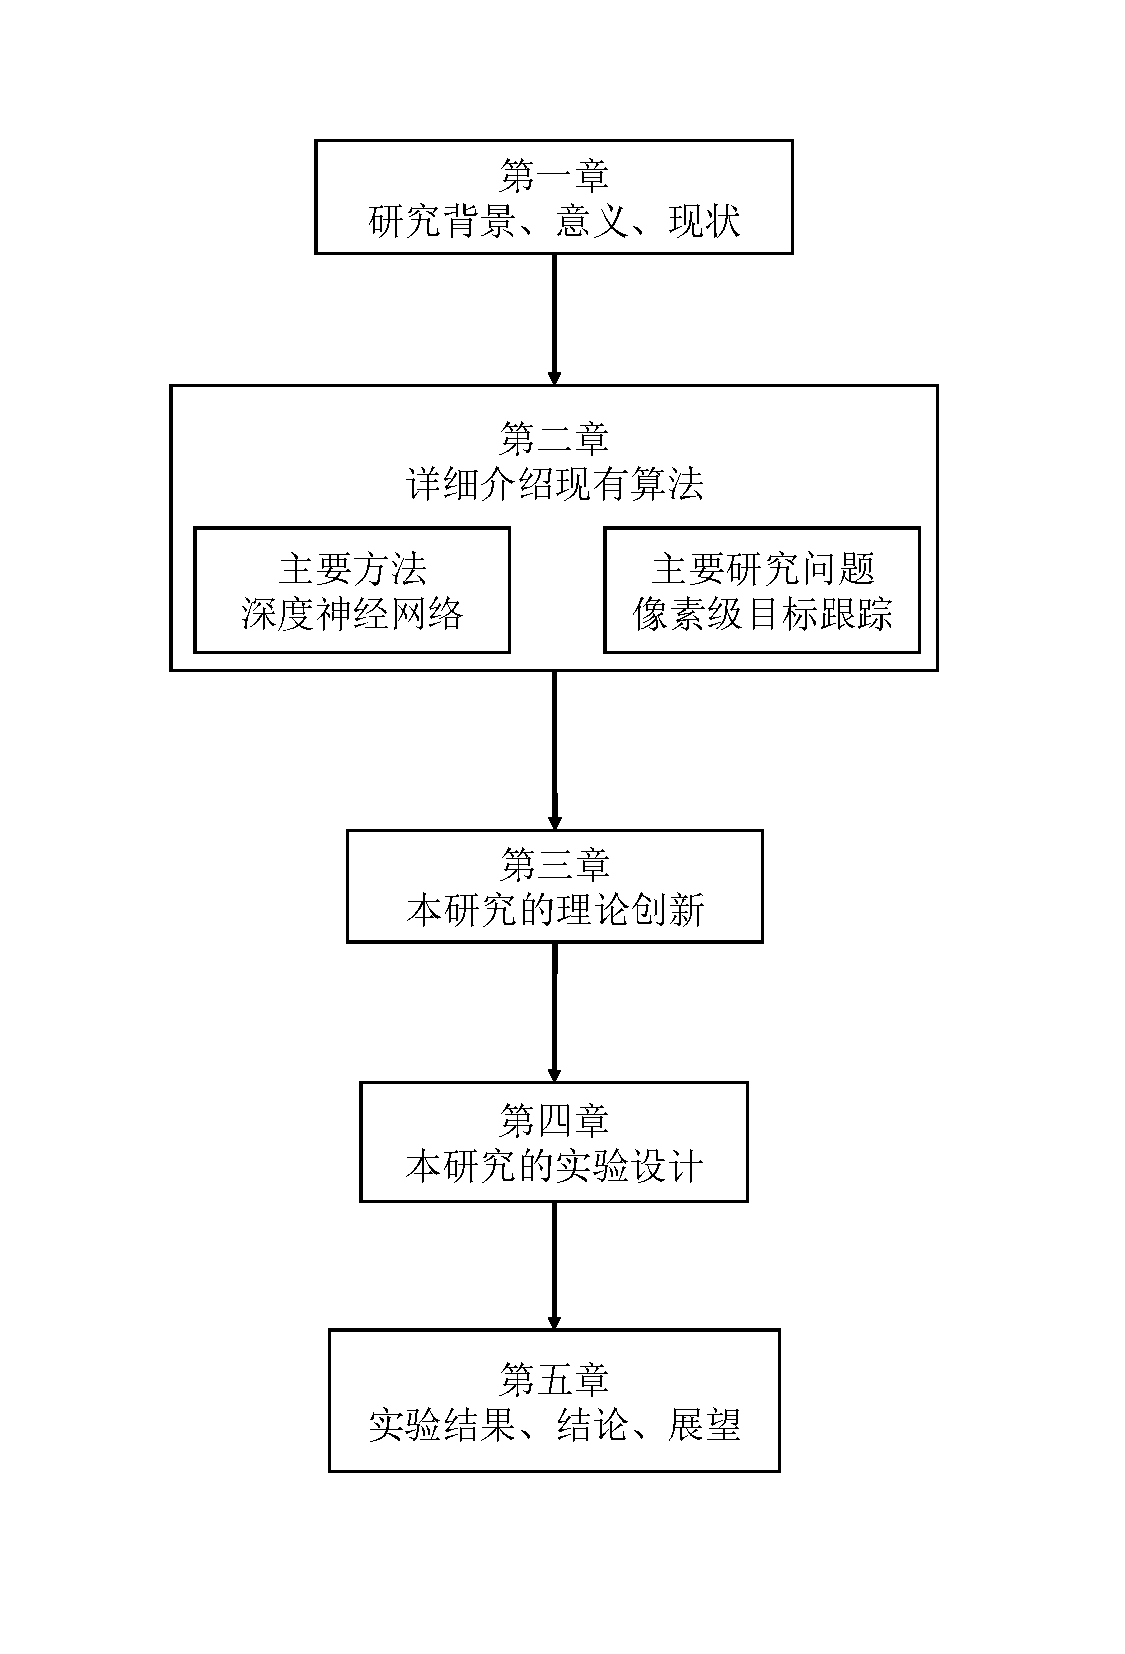
\includegraphics[width = .8\textwidth]{chap/img/thesis_structure.pdf}
    \caption{论文结构图}
    \label{fig:thesis_structure}
\end{figure}
\par
	% Copyright (C) 2019 Cui Jialiang ( SESS, PKU ). All rights reserved.

\chapter{深度学习理论与现有的视频目标跟踪算法概论}
本章将介绍深度学习与视频目标跟踪算法的基础概念与常用算法.
\par
深度学习是本研究运用的主要方法,但其并不是本人专业常用的方法.本研究为了利用计算机学最新的研究成果,研究并采用了计算机视觉,统计领域今年来常用的深度学习方法.本研究提出的算法也将主要由多种深度学习算法组合而成.
\par
本章还将介绍一些视频目标跟踪算法.
\section{深度学习基础概念}
深度学习(Deep Lrarning)是以深度神经网络为模型结构的机器学习算法\supercite{deng2014deep}.机器学习(Mechine Learning)通常指一些依靠计算机确定模型的建模方法.目前大多数机器学习算法还无法完全自行实现学习,通常只能在人为规定的模型下,针对某个小问题对特定的数据建模.
\par
机器学习,模式识别等学科最终试图解决的问题通常是建立模型,解决问题.如目标跟踪即可描述为输入是视频,输出是轨迹的问题.神经网络(Neural Network, NN)由于其优秀的非线性拟合能力,成为如今机器学习最常用的模型结构之一.
\subsection{神经网络}
神经网络最初的灵感一部分来源于仿生学\supercite{mcculloch1943logical}\supercite{farley1954simulation},这也是神经网络的灵魂思想.
\par
相比于k-NN,SVM(支持向量机),线性回归(linear regression)等传统机器学习算法,神经网络主要依靠激活函数(activation function)得到非线性效果.为了避免梯度消失的问题,近期的研究与应用中最常用的激活函数是ReLU激活函数\supercite{krizhevsky2012imagenet}.不同的激活函数会有不同效果\supercite{karlik2011performance}.
\par
而相比与各种树模型,神经网络又有更好的泛华能力.
\par
\subsubsection{全链接神经网络}
\par
最简单的神经网络结构是全连接的(Fully Connected, 简称FC)神经网络, 该结构又称多层感知机(Multi Layer Perceptron, 简称MLP).多层感知机由多个层$l_1,l_2,...l_n$依次排列组成.每个层由许多神经元组成,某以层上的每个神经元将接受上一层所有神经元为输入,并向下一层的所有神经元输出.以ReLU为激活函数,位第k层的第m个神经元的输出为$output_{k,m}=ReLU(\sum_{i} (output_{k-1,i}*w_{k,m,i})+b_{k,m})$,其中$w_{k}$和$b_{k}$是属于第k层的变量,通常经过训练得出.
\par
全连接神经网络的连接较多,参数也会更多,即所有参数组成的参数向量很稀疏,不利于训练.通常只在最终将多维的状态量收敛成低维结果时使用.在前期对高维的数据的处理过程中,常常会对神经网络的结构进行一定简化,减少连接以利于训练.常用的减少连接方式有卷积神经网络和循环神经网络等.
\par
\subsubsection{卷积神经网络}
\par
\begin{figure}[htbp!]
    \centering
    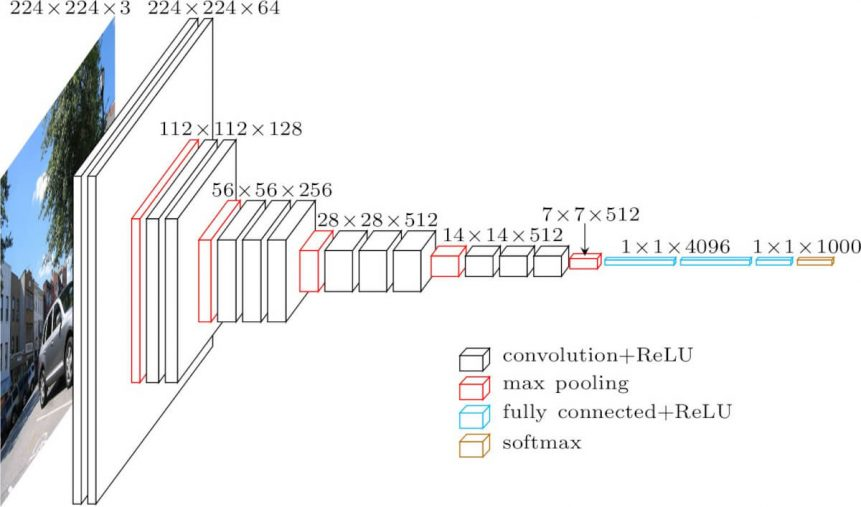
\includegraphics[width = 1.\textwidth]{chap/img/vgg16-neural-network.jpg}
    \caption{
        用于图像分类的VGG16\supercite{simonyan2014very}卷积神经网络结构图.图片来自 \url{https://neurohive.io/en/popular-networks/vgg16/}
        }\label{fig:vgg16_architecture}
\end{figure}
\par
卷积神经网络(Convolutional Neural Network, 简称CNN)是一种为图像处理设计的神经网络结构.同全连接神经网络一样,卷积神经网络也分为很多层,每一层只与前一层和后一层连接.不同的是,每层的一个神经元只连接前一层与后一层的少部分神经元.通常,CNN的每一层可以用一个多波段图像表示,连接只建立在前一层与后一层位置接近的像素上.类似图像处理中的模板滤波方法.常用的CNN的模板大小是$3*3$,有时也可以是$5*5$,$7*7$等大小.每一层的所有神经元公用一个模版,模版上所有的参数都是训练得到的变量.卷积神经网络同样要在每层上加入激活函数,常用ReLU激活函数.
\par
完整的卷积神经网络通常会在卷积层中穿插池化(Pooling)层以收敛数据维度.池化层可以将卷积层图片大小减小.常用的配合ReLU激活函数的池化层如最大值池化(Max Polling)方法.以$2*2$为池的大小的池化层的输出为输入层大小的一半,每个像元为对应位置的4个像元的最大值.
\par
以图像分类问题为例,该问题需要输出一个较低维度的结果,即图像属于是每个类别的概率,可以用一个向量表示.用于图像分类的神经网络通常使用CNN层与最大值池化层交替减小图像大小,最终用全连接层得到分类结果.如图\ref{fig:vgg16_architecture}所示的VGG16\supercite{simonyan2014very}卷积神经网络即是这样一个图像分类算法.
\par
\begin{figure}[htbp!]
    \centering
    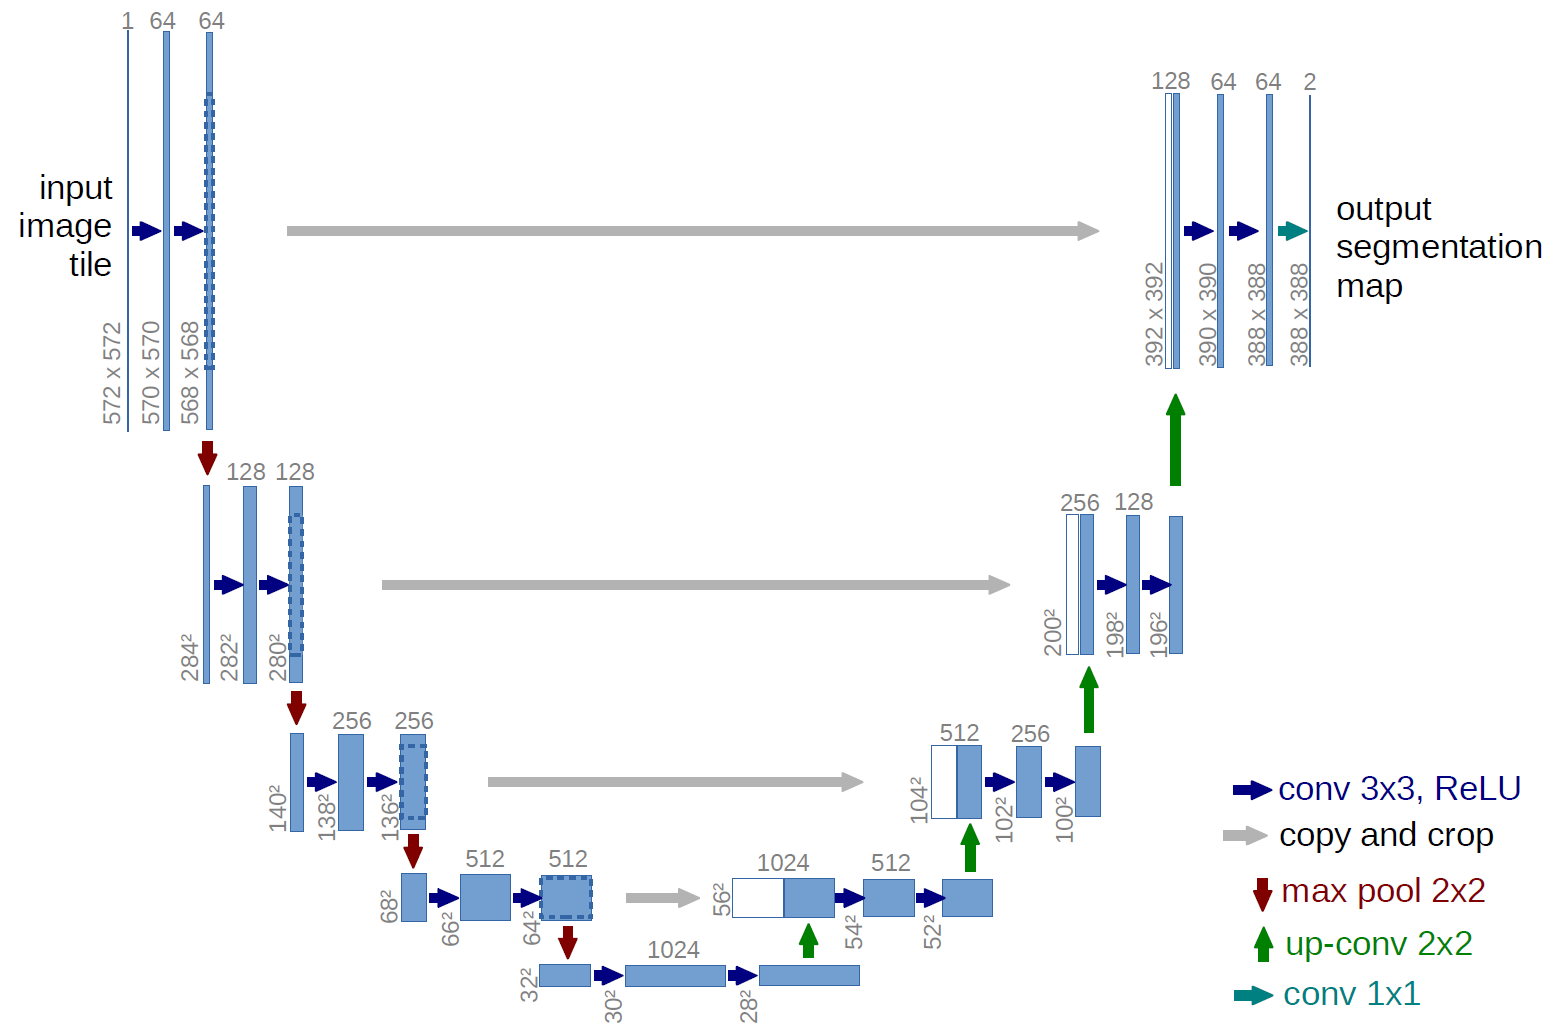
\includegraphics[width = 1.\textwidth]{chap/img/u-net-architecture.png}
    \caption{
        用于图像分割的U-Net\supercite{ronneberger2015u}卷积神经网络结构图.
        }\label{fig:unet_architecture}
\end{figure}
\par
不同于图像分类,图像分割等像素级图像处理问题需要得到更高维的结果,且得到的结果需要有一定的空间特性.如图\ref{fig:unet_architecture}的U-Net是一种常用的处理分割等像素级别问题的卷积神经网络.该网络有加密和解码两个步骤,加密阶段图像经过多次卷积和池化变小,蕴含的信息更宏观;而解码阶段图像经过反卷积(Deconvolution)操作再次放大,得到与原图大小相似的结果.类似的还有SegNet\supercite{badrinarayanan2017segnet}卷积神经网络等.
\par
U-Net的网络结构为像素级别处理提供了思想基础.
\par

\subsubsection{循环神经网络} \label{section:rnn}
RNN(循环神经网络, 又称递归神经网络, Recurrent Neural Network)是深度学习处理序列问题,尤其是时间序列数据时的重要方法.上文中介绍了全连接和卷积神经网络,这两种结构的神经网络接受的输入都是由网络结构事先确定的.如针对图像处理问题,通常的做法是将图片采样,拉伸至CNN的输入要求再进行处理.当进行时间序列分析时,这样的结构只能接受定长的时间序列数据.但实际上大多数时间序列数据是变长的.
\par
\begin{figure}[htbp!]
    \centering
    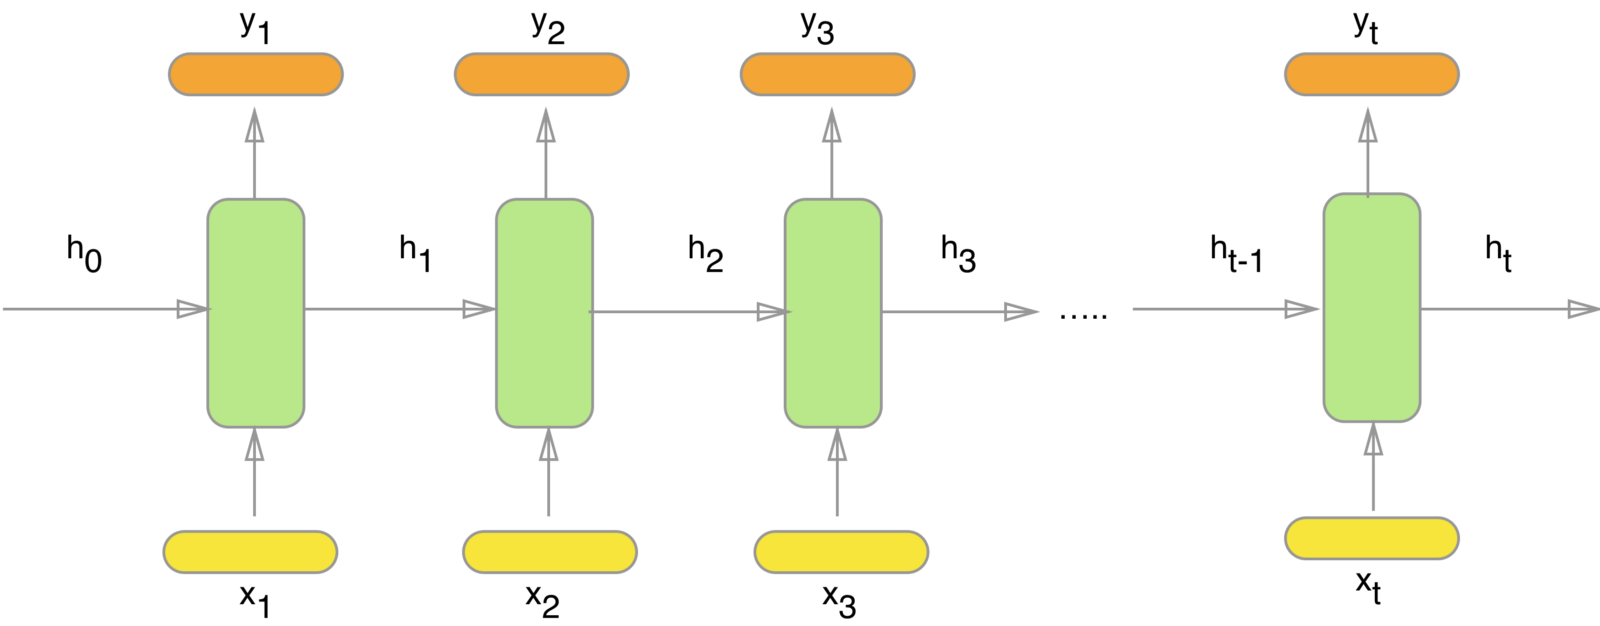
\includegraphics[width = 1.\textwidth]{chap/img/rnn.png}
    \caption{
        RNN的输入$x$,输出$y$与状态$h$的结构\supercite{how_rnn_work}
        }\label{fig:rnn}
\end{figure}
\par
RNN能很好解决这个问题.RNN可以将参数相同的某个神经单元重复使用多次以处理.通常情况下\footnote{这里介绍的RNN全是单向RNN,且对时间序列处理的先后顺序为时间流逝的顺序},RNN单元接受前一时刻的状态量和本时刻的信息,得到本时刻的输出和输出给下一时刻的状态量.
\par
如图\ref{fig:rnn}所示,对一个长度为$t$的时间序列,我们在每个时刻观察到的信息为$x_1, x_2, ...x_t$,则对第$i$时刻,有$y_i,h_i = RNN(x_i, h_{i-1})$.其中$y_i$为该时刻处理得到的结果,$h_i$为该时刻的状态描述即状态量,$RNN$为该RNN的处理函数,该RNN对每个时刻的处理函数参数相同.通常情况下,$x,y,h$都是张量.
\par
RNN可以得到和原序列一样变长结果,也可以得到定长的结果.通常变长的结果由每时刻的输出即上段的$y$组合得到,而定长的结果由最终的状态$h_t$经过处理得到.定长的结果一般用于该序列进行一个系统的描述,而变长的结果需要得到该序列每个时刻的信息.
\par
%TODO 介绍LSTM
%TODO 介绍RNN展开方式

\subsubsection{用于分类问题的神经网络结构}
\par
无论是FC,CNN还是RNN结果,神经网络在处理过程中传递的都是张量(Tensor\footnote{著名的深度学习框架Tensorflow\supercite{abadi2016tensorflow}即得名于此}).常见的矩阵(Matrix),向量(Vector)都是张量.如FC神经网络处理某条数据时,神经元数位$k$的某一层传给下一层的信息可以用大小为$k*1$的张量表示.这是这个量是一个向量.
\par
\begin{figure}[htbp!]
    \centering
    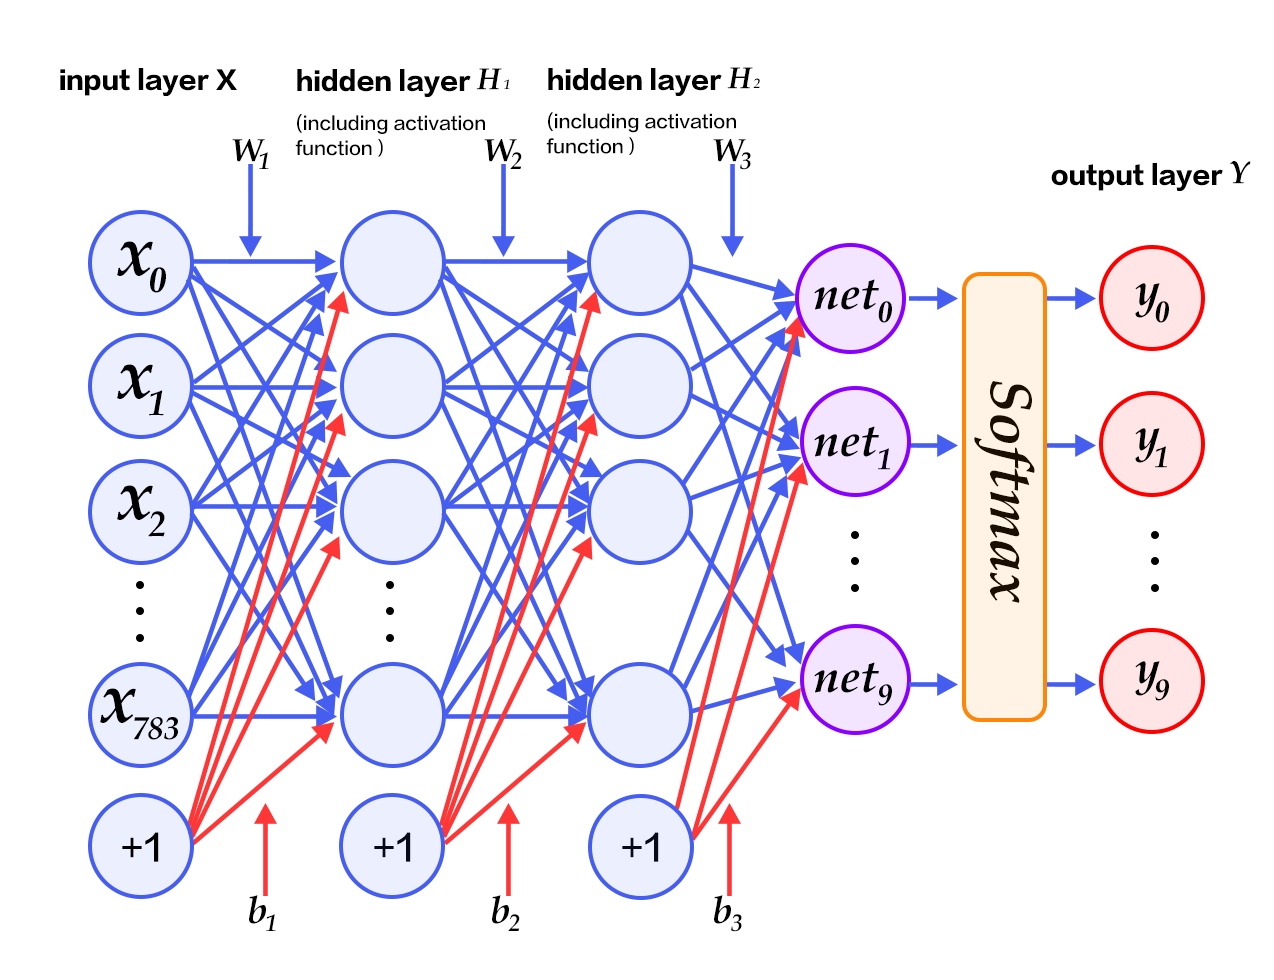
\includegraphics[width = 1.\textwidth]{chap/img/mlp_paddle.png}
    \caption{
        使用Softmax实现分类的多层神经网络,图片来自百度公司PaddlePaddle平台(\url{https://github.com/PaddlePaddle/Paddle})的文档\supercite{recognize_digits_paddle}
        }\label{fig:mlp_paddle}
\end{figure}
\par
图\ref{fig:mlp_paddle}即是一个用于分类问题的神经网络.


\subsubsection{深度神经网络的训练}
\par
\begin{figure}[htbp!]
    \centering
    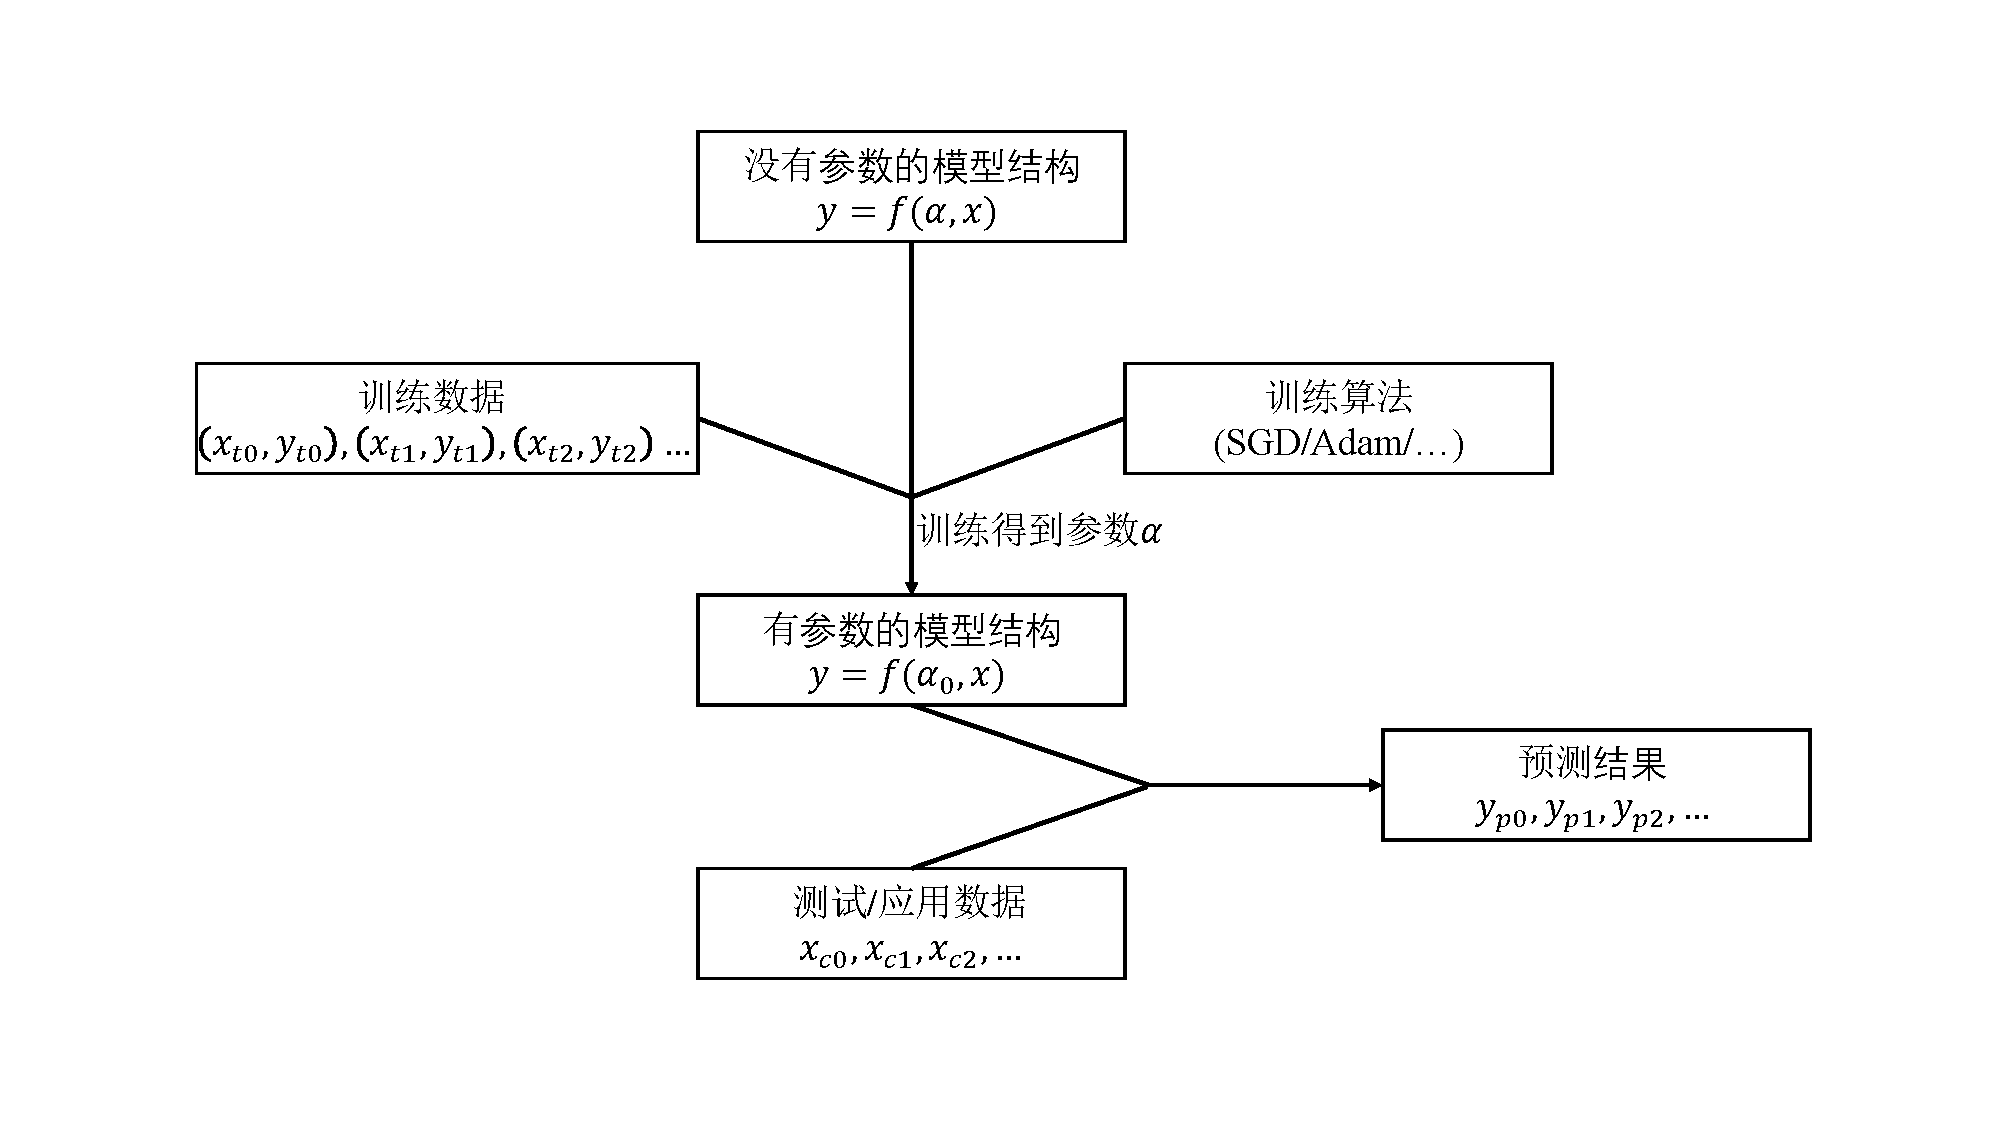
\includegraphics[width = 1.\textwidth]{chap/img/model_learning.pdf}
    \caption{使用训练数据,将没有参数的模型$f(\alpha,x)$训练至有参数,可以实际应用的模型$f(\alpha_0,x)$的过程}
    \label{fig:model_learning}
\end{figure}
几乎所有的深度神经网络都需要配合训练(training)得到的参数才能应用,即预测.不同的训练会得到不同的参数,预测得到的结果也会不同.
\par
梯度下降法是最典型的模型训练方法.
\par
反向传播是常用的深度神经网络求梯度的方法.

\section{视频跟踪算法}
上一章中介绍过,视频跟踪算法接受图像序列,输出目标位置.具体的,对于一个$n$帧长的,由$pic_1,pic_2...pic_n$共$n$张图像组成的视频,使用跟踪算法$Track$进行跟踪,在第$t$时刻算法的计算可以用下面的公式表示:
\par
\begin{equation}\label{equ:track_ite}  P_t,S_t=Track(pic_{t},P_{t-1},S_{t-1})  \end{equation}
\par
其中$P_t$,$S_t$分别代表$t$时刻的\textbf{目标位置与形态}和\textbf{跟踪状态}.这两个概念将在本节后边介绍.
\par
在整个跟踪过程中,跟踪系统将在每一帧到来时执行公式\ref{equ:track_ite}中描述的过程,最终获得所有的目标位置与形态$P$.
\par
\subsection{目标位置与形态的描述} 
所有目标跟踪算法都有明确的\textbf{目标位置与形态的描述}方法.事实上,这种描述基本可以等同于目标跟踪算法的输出形式.典型的目标位置与形态描述有矩形式和像素级的.
\par
\subsubsection{矩形式目标位置与形态描述}
\par
\begin{figure}[htbp!]
    \centering
    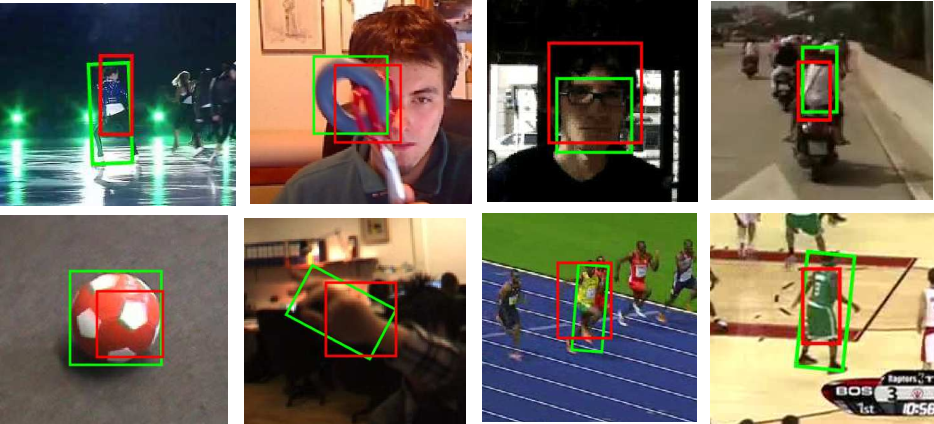
\includegraphics[width = 1.\textwidth]{chap/img/overlap_examples.pdf}
    \caption{图片为VOT竞赛中描述标记与目标的插图\supercite{VOT_TPAMI},这里用于演示矩形式目标描述中描述目标的外包矩形.红色:限定竖直的的外包矩形;绿色:不限定竖直的外包矩形.}
    \label{fig:bunding_boxes}
\end{figure}
\par
常见的矩形框视频目标跟踪算法考虑会考虑目标的最小外包矩形(Bounding Box)和位置(Location).最小外包矩形的方向有时是限定为竖直的,即矩形的上下边平行于图像的上下边,左右边同理;有时不限定,可以是任何方向.限定竖直与不限定竖直的矩形表示法如图\ref{fig:bunding_boxes}所示.位置一般用矩形的中心表示.
\par
\subsubsection{像素级目标位置与形态描述}
像素级跟踪算法的运动模型需要表达的信息与矩形框跟踪算法类似,但信息更为细节.像素级目标描述没有矩形式目标描述那样用矩形的中心描述目标的位置,用矩形的形状描述目标的形状.而是直接用二值的,覆盖全图的像素来同时描述目标的位置与形状.
% TODO 此处应有图演示像素级描述方式

\subsection{跟踪状态}
\textbf{跟踪状态}是跟踪模型在跟踪过程中,用于记录当前信息以继续跟踪的状态量.在$t$时刻的跟踪状态$S_t$,它的物理含义可能包含用于预估目标将来的运动的目标之前一段时间的运动与变化状态.通常情况下,跟踪模型预测新一帧的目标位置需要用该帧到来时刻的跟踪状态与该帧的图像,但如果跟踪状态描述得足够理想,很多情况下仅凭描述优秀的跟踪状态就可猜测出目标接下来的运动趋势,从而大致确定新的目标位置与形态.
\par
多数基于深度学习的视频目标跟踪算法都使用RNN的状态量存储目标跟踪状态.
\par

% TODO 介绍经典跟踪算法
	\chapter{基于CNN和RNN的像素级别跟踪算法}
本章是本文的重点,将详细介绍本研究的理论创新。
\par
本研究提出一种结合现有的像素级别处理技术和现有的矩形级视频目标跟踪技术的像素级别目标跟踪算法,具体算法结构,实现细节,训练等将在本章重点介绍.
\section{算法结构与核心思想}
本文所实现的算法将首先基于用于实现静态图像分割的U-Net\supercite{ronneberger2015u}的多级降级-升级卷机神经网络结构.但将在这个多级网络结构中加入Conv-LSTM结构.
\par
类似与U-Net的结构,本文的卷机网络部分也将有多个降级和升级结构;每个降级结构包括几个卷积层,使用池化结构进行降级;每个升级部分采用升卷积进行升级处理.在降级过程中,图片数据的尺寸大小会衰减,同时等比例增加其波段范围.对于3层的结构,最小级的波段将有128个.这个多级结构的设计理念是为了处理多尺度问题;浅层的级别能很好的处理细节问题,但对宏观的把控会较弱,具体表现为可能会出现噪声点;深层的结构对宏观把控好,但对边界处理较弱.升级结构能将浅层处理得到的边界信息与深层处理得到的宏观信息相结合,得到一个更好的结果.
\par
在时间尺度,本研究的算法将主要采用LSTM算法解决问题.具体的,LSTM单元将被加入到各个层级当中.LSTM在各种跟踪算法中有广泛应用,但大多数算法仅仅将其作为对最后结果的处理手段.本研究的算法将把LSTM作为所有的中间状态记录单元.
\par
与纽约大学2017年实现的Conv-LSTM结构的跟踪算法不同的是,本文所采用的多级神经网络将把Conv-LSTM加入各个卷机层级;而与U-Net,SegNet等多级分割算法不同的是,本文将在整个结构中多处穿插LSTM以得到一个时间连续的结果.
\section{基于CNN和RNN的像素级别跟踪模型在空间维度的处理}
\subsection{CNN的原理}
\subsection{多尺度思想的引入}
\section{基于CNN和RNN的像素级别跟踪模型在时间维度的处理}
\subsection{RNN的原理}
\subsection{跟踪状态}
\subsection{跟踪系统初始化}
\section{模型训练}
\subsection{机器学习思想}
\subsection{模型训练原理}
	% Copyright (C) 2019 Cui Jialiang ( SESS, PKU ). All rights reserved.

\chapter{基于Tensorflow的像素级视频目标跟踪实验} \label{section:experiment}
为了验证本研究提出的方法的可行性和价值,我们设计了一个实验.后文中该实验将被称为本实验.本实验基本实现了本研究提出的方法,并得到了一定的结果和结论.
\par
本章接下来的部分将介绍本实验的设计思路,硬件环境和数据等实验条件,实验代码的实现和实验结果的评估方法.

\section{实验总体设计思路}
类似于大多数算法研究,本研究以计算机软件的形式实现了本研究提出的算法,并选择数据进行了实验.

\section{实验软硬件环境}
\subsection{软件环境}
本实验的软件部分主要在Tensorflow\supercite{abadi2016tensorflow}框架下实现.
\par
Tensorflow是最初由谷歌公司开发的一套现以开源的机器学习框架,可以为算法研究者提供屏蔽操作系统与硬件,资源分配,梯度计算等功能,让研究者能将更多的注意力集中在算法过程中.对于本研究,Tensorflow主要贡献了CNN,RNN单元的结构定义,损失函数定义,正向反向传播与梯度更新等功能.

\subsection{硬件环境}
\par
需要说明的是本研究提出的算法可以部署在普通计算机上,也有希望部署在更快速,更低成本的FPGA等嵌入式平台上.本实验为了容易进行,目前只在PC(个人计算机)上进行.
\par
本实验所有的运算操作是在一台配置有英伟达GTX1070图形处理器,英特尔i7中央处理器,24GB内存的笔记本电脑上进行的.
\par
本实验深度学习计算部分使用了GPU加速,直接依赖Tensorflow的GPU选项进行.本研究曾尝试过只用CPU进行计算,也能得到一定结果.
\par
如果有更好的硬件条件(更多、更好的图形处理器,更大的内存,更多核心的CPU),本实验有希望会得到更精细的结果.

\section{实验数据}
本实验使用VOT2016数据集\supercite{Vojir-TR-2017-01}实现,相似的数据集还有VOT2017等.
\par
\begin{figure}[htbp!]
    \centering
    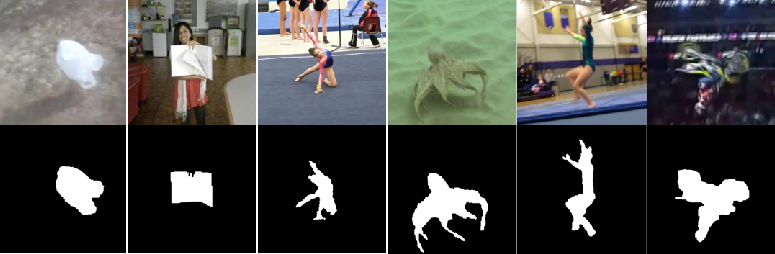
\includegraphics[width = 1.\textwidth]{chap/img/vot_2016_pixel.png}
    \caption{VOT2016像素级标记}\label{fig:vot_2016_pixel}
\end{figure}
\par
如图\ref{fig:vot_2016_pixel}所示,该数据集通过人工标记,提供了十分优秀的像素级的目标跟踪数据.该数据集有几百个序列,共有几万张图片.
\par
本实验的训练集和测试集均来源于该数据集,使用时将所有数据随机切分为训练集和测试集.
\subsection{Ground truth}
Ground truth是一个机器学习中的概念,意为根据某种参考得到的标注数据.尤其是在图像领域,所有的参考都不能被肯定是完全正确的,ground truth就指这样的标注结果.大多数ground truth可以有很强的正确性,如大多数人工标注的图像训练数据,其正确程度已经可以用于机器学习训练,但在一些边界区域还是会有一些人工操作导致的误差.

\section{实验程序的编写}
事实上,虽然借助于Tensorflow实现了许多计算功能,但本研究依然经历了许多代码开发工作,包括且不限于神经网络结构定义,训练数据处理等.
\par
本实验现先定义了CRNN的结构,即输入一个时间序列的序列图像,经过CRNN卷机循环网络得到另一个结果时间序列.在本实验的程序中,该结构可以选择使用LSTM或普通RNN单元.
\par
在加密-解码结构中,本实验定义了一个通用的层级结构,可以重复使用多次.如重复3次即是3层加密-解码结构.

\section{实验结果的评估方式}
由于像素级的视频目标跟踪算法缺乏评估体系,本实验直接将跟踪问题视为像素级二分类问题,用二分类问题的评价方式来评价实验结果.
\par
% TODO 混淆矩阵
对于像素级跟踪问题,分类结果中所有像素可以分为分类得到的正例(目标)和负例(背景),同样的,ground truth中标记的像素也可以分为正例和负例.
\par
对于ground truth中标记为正例和负例的像素,分别被分成正例和负例可以用混淆矩阵表示
\subsection{分类问题评估:准确率和召回率}
准确率(accuracy)和召回率(recall)可以用于描述分类问题的精确程度.
\par
准确率指分类器将结果分对的概率,将正例分为正例,将负例分为负例都是分对.在本实验中,准确率可以衡量一个跟踪算法大体上对结果的正确估计率.但如果在一个场景中目标较小,将所有像素分为背景的算法依然能得到很高的准确率.
\par
\begin{equation}\label{equ:accuracy}  Accuracy=\frac{TP+TN}{TP+FP+TN+FN}  \end{equation}
\par
召回率指正例结果的正确性,即结果中的正结果,其是本来就是正例的概率.该衡量方式避免了准确率带来的问题,但只能估计目标,无法确定背景的预测准确定.
\par
\begin{equation}\label{equ:recall}  Recall=\frac{TP}{TP+FN}  \end{equation}
\par
上述准确率与召回率用于评估带来的问题是大多数二分类问题(如点击率预估等)中必然存在的.本文使用AUC评估方法解决这个问题.

\subsection{分类问题评估:AUC} \label{section:auc}
%TODO ROC介绍
AUC的一种直观定义是对于groundtruth中的任一个正例$a$和任一个负例$b$,分类系统认为$a$比$b$更像负例的概率.该评价方式能较好的中和准确率和召回率带来的问题.通常AUC达到0.9以上就可以认为是很好的分类结果.
\par
对于一个很多张图组成的视频,本实验先分别评价每张图的AUC,再做平均得到整个视频序列的AUC.
\par
需要注意的是,如果直接对整个视频序列求AUC,会出现前后置信度不同的问题.由于跟踪预估得到的是预计像素属于跟踪目标的概率,对于不同场景的不同帧概率基准可能不同,得到的结果也会不准确.
\par
除了需要关注整个视频的平均AUC,还需要关注AUC的衰减.由于信息的丢失,在一开始的跟踪中跟踪往往是最准确的,随着跟踪时间的推移,跟踪信息会逐渐损耗.更好的跟踪系统损耗会更慢.
	% Copyright (C) 2019 Cui Jialiang ( SESS, PKU ). All rights reserved.

\chapter{结果,结论与讨论}
本章将主要介绍本文为验证本文的实验(见\ref{section:experiment})的结果,本研究的结论,与本研究引发的讨论.
\section{实验结果与结论}
本研究的实验顺利进行了,并得到了结果.
\subsection{实验结果图像展示}
\par
\begin{sidewaysfigure}[htbp!]
    \centering
    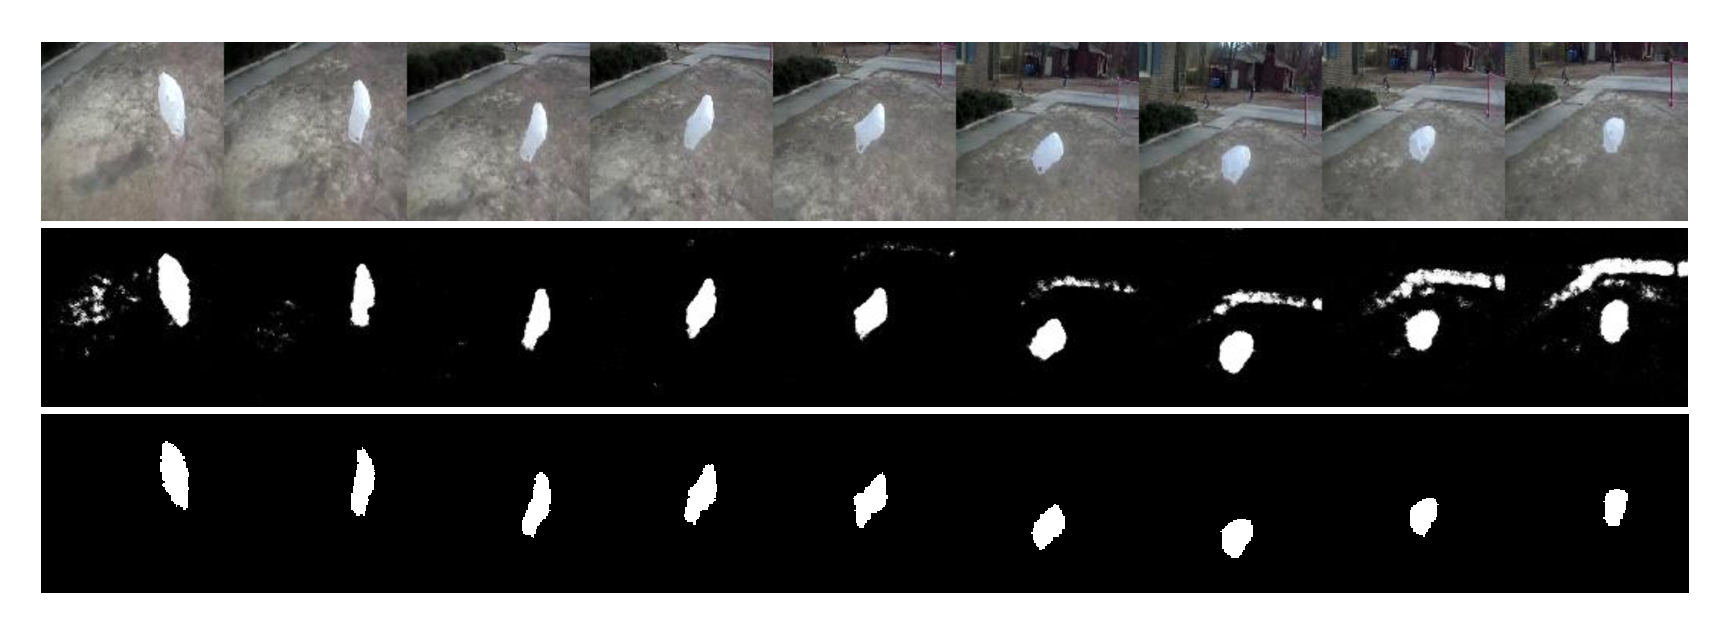
\includegraphics[width = 1.\textwidth]{chap/img/result_bag.pdf}
    \caption{跟踪结果-袋子:第一行为原图,第二行为跟踪结果概率图,第三行为二值化结果}
    \label{fig:result_bag}
\end{sidewaysfigure}
\par
\begin{sidewaysfigure}[htbp!]
    \centering
    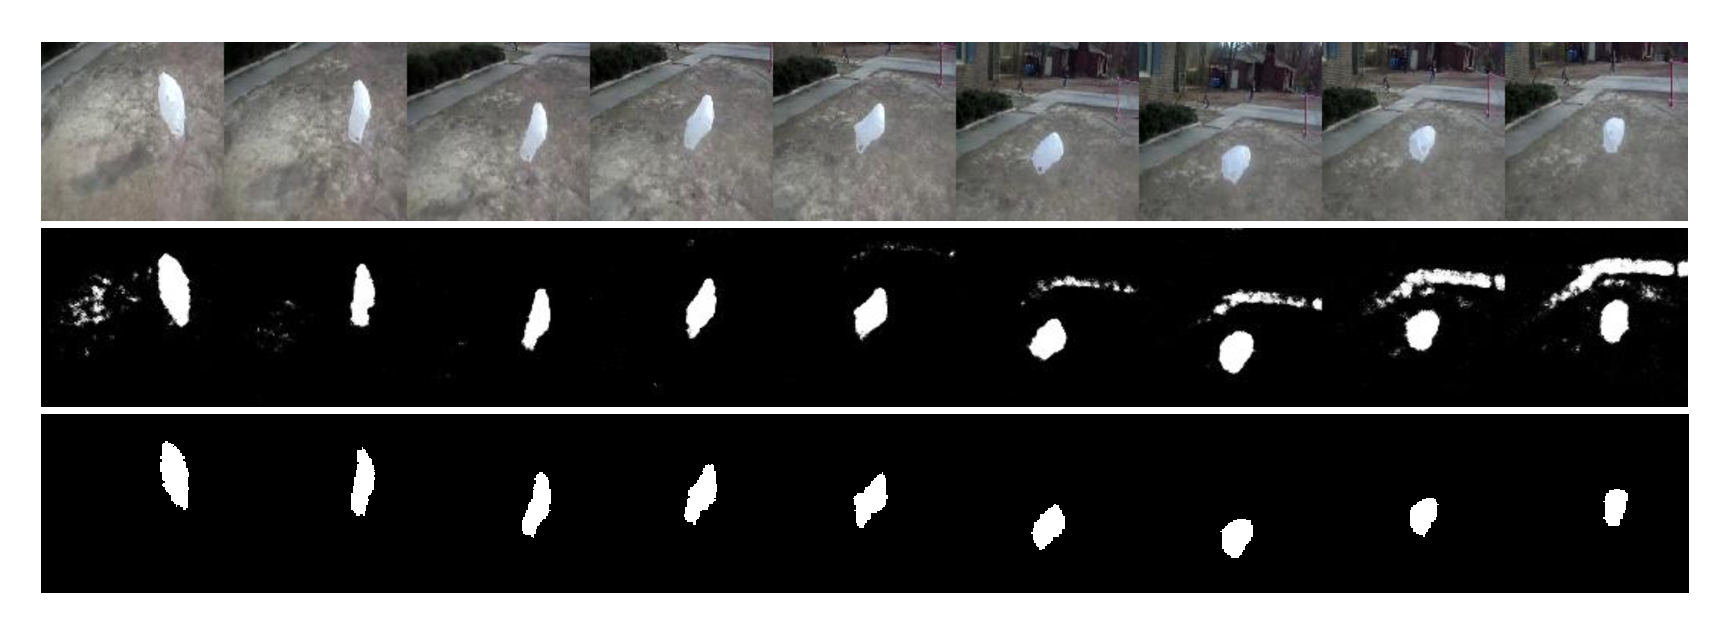
\includegraphics[width = 1.\textwidth]{chap/img/result_bag.pdf}
    \caption{跟踪结果-老虎玩具:第一行为原图,第二行为跟踪结果概率图,第三行为二值化结果}
    \label{fig:result_tiger}
\end{sidewaysfigure}
\par
实验结果的图像展示见图\ref{fig:result_bag}和图\ref{fig:result_tiger}.
\par
\subsection{实验结果定量评估}
\par
\begin{sidewaysfigure}[htbp!]
    \centering
    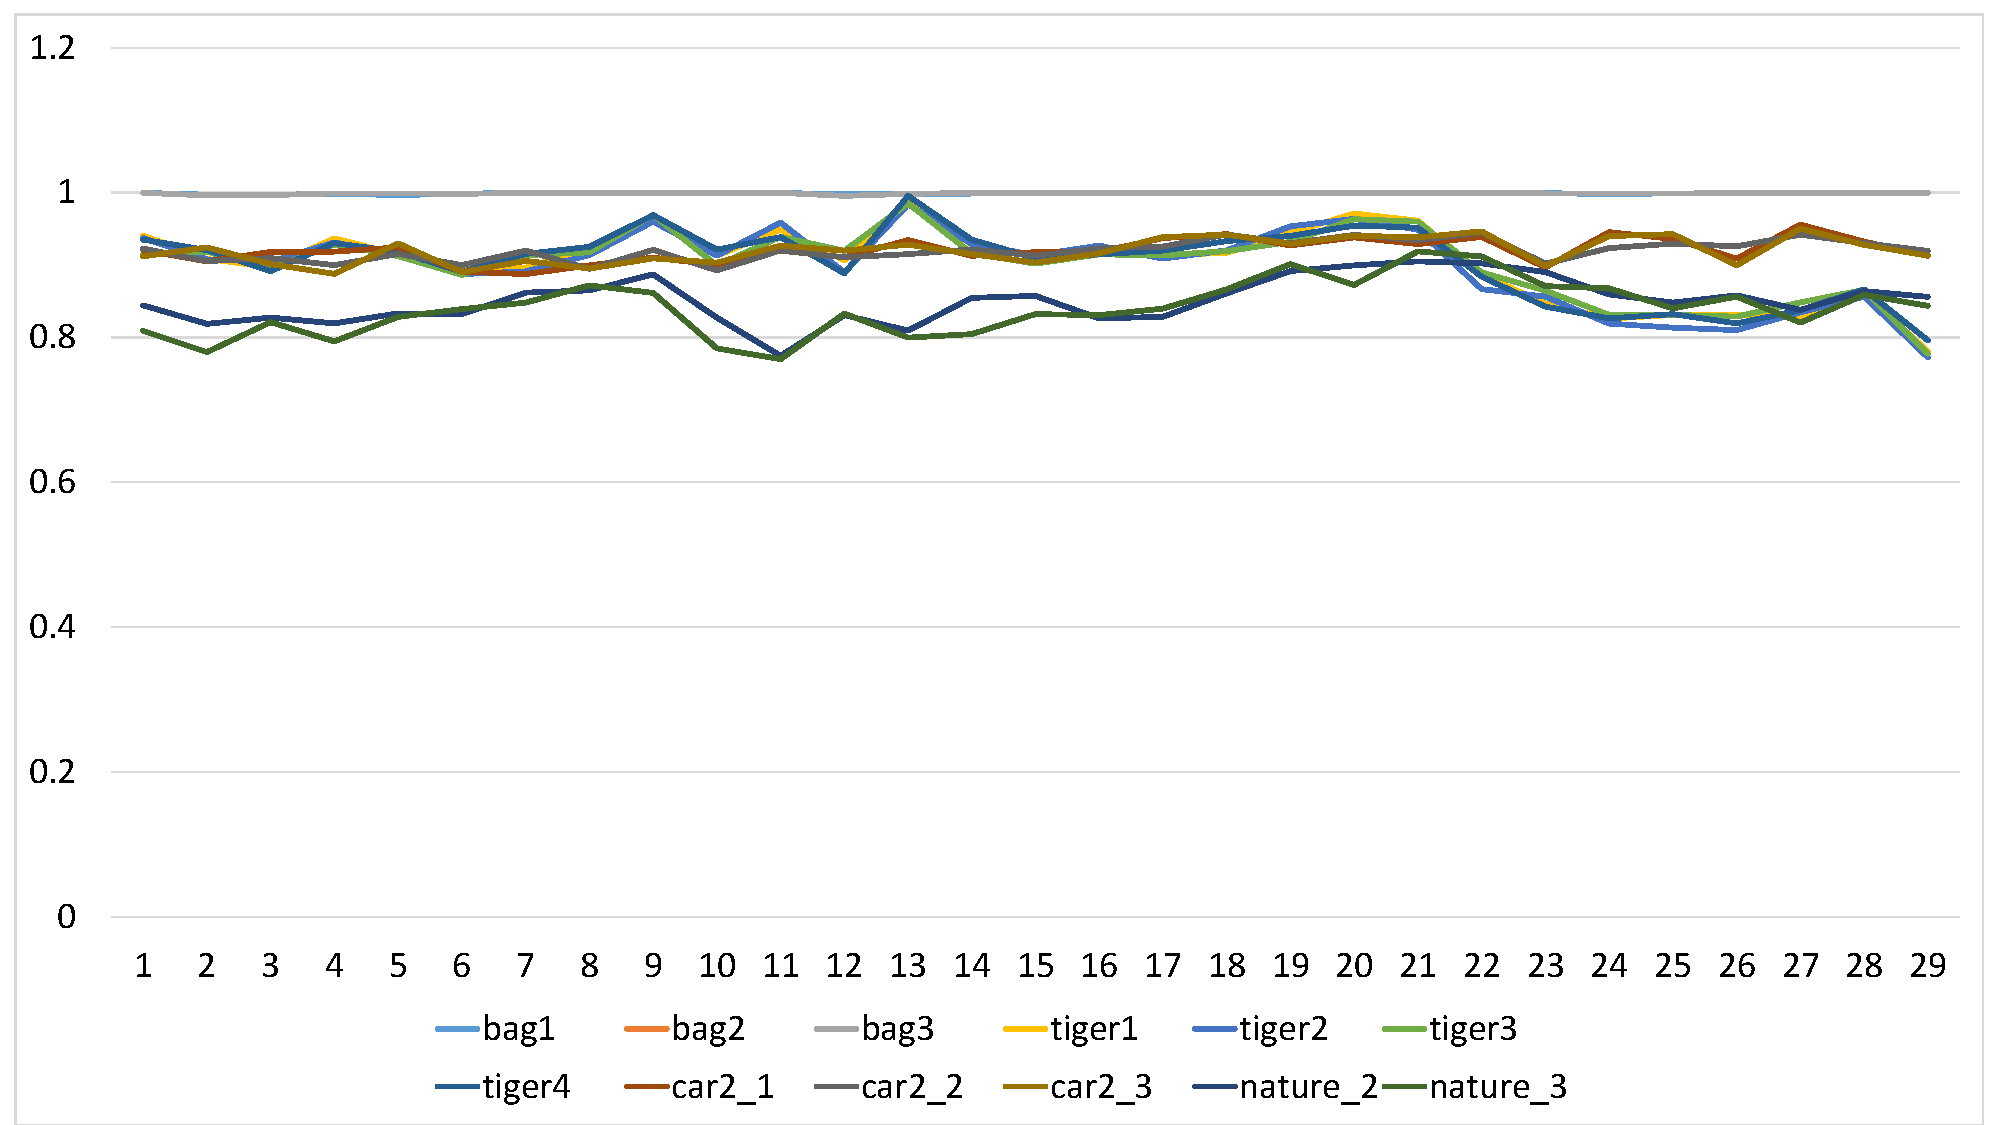
\includegraphics[width = 1.\textwidth]{chap/img/res_auc.pdf}
    \caption{测试集中一些序列的跟踪AUC统计}
    \label{fig:res_auc}
\end{sidewaysfigure}
\par
本实验采用了AUC作为评价结果(详见前文\ref{section:auc}).图\ref{fig:res_auc}中展示了几组实验的AUC统计.
\par
可以看到,在许多样本序列中,本研究的模型具有一定的跟踪能力.
\subsection{实验结论}
经过实验,本研究提出的像素级目标跟踪算法具有一定的像素级目标跟踪能力,具有应用的前景与希望.

\section{总结与讨论}
本节将总结研究的结论,分析并罗列本研究的创新点与不足,并对接下来的工作进行展望.
\par
本研究提出了一种基于CNN和RNN的像素级目标跟踪算法,主要运用了深度学习技术中的循环神经网络与加-解码结构;实现并用数据进行了实验,得到了较好的实验结果.
\subsection{本研究的创新点}
本研究第一次在有物理依据的情况下将RNN插入加密-解码结构的各个层级.这种结构对于处理多尺度图像处理问题将有创新效应.过去的研究中CNN与RNN的结合方式大多是先用CNN得到向量结果,再用RNN对这个结果进行处理.本文的思路会为RNN保留更多的空间信息.
\par
近年来像素级别的跟踪一直缺乏研究,而像素级的跟踪更加贴近跟踪本质.本研究的进行有利于推动像素级跟踪算法的研究与迭代.
\subsection{本研究的不足}
由于数据集的限制,本研究实验时采用的训练与测试数据序列都太短,还未达到实际应用需要的长度.这需要更长视频的数据集的支持.
\par
本研究进行的实验较有限,一方面受数据集的范围限制,另一方面受硬件限制,无法进行更大规模的训练.本研究将图像采样至$500*500$大小,实际上是由于平台内存不足的无奈之举.如果输入图像可以更大,像素级跟踪得到的结果就会更精致,处理过程中的信息损失也会更小.
\par
也由于平台与实验时间限制,本研究的实验只实现了3层的加密-解码结构.目前通常图像分割会采用5层以上的加密-解码结构,以保证深层的CNN能获取更加全局的信息.本文虽然使用Conv-LSTM结构处理了全局信息,但如果能在加密-解码结构中增加更多的全局信息,将对解码过程有巨大的帮助.
\subsection{后续工作}
本文的后续工作将在以下几个方面进行:
\begin{itemize}
    \item 添加更多数据,得到更多实验结果.
    \item 尝试更深层次的加密-解码结构,与更大的初始图像处理.
    \item 尝试真实应用场景的数据的跟踪效果.
    \item 尝试调整模型参数以求得到更好的效果.
    \item 尝试微调模型结构,如加密-解码结构与RNN的结合层数等.
    \item 尝试该结构(RNN加入各级加密-解码结构)在其它问题,如视频目标分割,视频稳定\supercite{benchme}等场景的应用.
\end{itemize}

\subsection{展望}
本文证明了加入了RNN结构的加密-解码模型在像素级目标跟踪问题上的效果,也发掘了像素级别目标跟踪问题的研究空间.根据目前的研究趋势,像素级以及矩形级的目标跟踪的推动都主要依靠深度学习算法.
\par
近期的深度学习研究主要在修改深度神经网络的模型结构,以求得到更适应问题的神经网络,并得到更好的结果.神经网络结构的改进包括基础网络单元,如CNN,RNN,以及本文的块状CNN,也包括各种基础网络单元结构的组合方式.
\par
对于跟踪问题,本研究中认为迫切需要解决的网络结构问题有:
\begin{itemize}
    \item 更好的RNN单元,更能保留有效信息,更好的长效处理.
    \item 更有效的RNN与CNN结合方式.
    \item 更多的神经元,容纳更多模型参数,得到更泛化的结果.
\end{itemize}
\par
但在模型结构,训练方法,数据集等问题逐渐完善后,深度学习算法何去何从,如何产生更加优于当前解法的模型将是一个问题.一些学者研究了网络结构的学习\supercite{cortes2017adanet},试图使用计算机替代人类进行网络结构的调整,这样可以使网络结构调整进入'工业化'阶段,大大提高效率.但也有人担心这样容易过早形成强人工智能\supercite{kurzweil2005singularity},对人类生存带来威胁.

% vim:ts=4:sw=4


	% 正文中的附录部分。
	\appendix
	% 排版参考文献列表。bibintoc 选项使“参考文献”出现在目录中;
	% 如果同时要使参考文献列表参与章节编号,可将“bibintoc”改为“bibnumbered”。
	\printbibliography[heading = bibintoc]
	% 各附录。
	%% Copyright (c) 2014,2016 Casper Ti. Vector
% Public domain.

\chapter{附件}
\pkuthssffaq % 中文测试文字。

% vim:ts=4:sw=4


	% 以下为正文之后的部分,默认不进行章节编号。
	\backmatter
	% Copyright (C) 2019 Cui Jialiang ( SESS, PKU )。 All rights reserved。

\chapter{在学期间发表的学术论文和成果}
\begin{itemize}
    \item[ {[}1{]} ] 崔家梁,冯朝晖,李芹,赵红颖. 基于CNN和RNN的像素级视频目标跟踪算法. 全球定位系统(已录用,中文核心).
\end{itemize}
% vim:ts=4:sw=4
	% 致谢。
	% Copyright (C) 2019 Cui Jialiang ( SESS, PKU )。 All rights reserved。

\chapter{致谢}
首先诚挚的感谢我的导师赵红颖老师,赵老师悉心的教导使我得以一窥数字图像处理领域的深奥,不时的讨论并指点我正确的方向,使我在这些年中获益匪浅。赵老师对学问的严谨更是我辈学习的典范。在此,我向我的指导老师表示最诚挚的谢意!本论文的完成另外亦得感谢实验室的冯朝晖,李芹,刘旭林同学和已经毕业的师兄师姐们的协助。因为有你们的帮忙,本论文能够更完整而严谨。
\par
感谢父母在我研究生期间对我的支持。
\par
感谢我的室友李昊远,胡安冬,王雯,几年同寝,无数次开黑,你们的帮忙我铭感在心。感谢在山鹰社遇到的志同道合的朋友们,愿鹰们能继续远走高飞。
\par
本论文在写作过程中使用了Overleaf在线编辑器 \url{https://www。overleaf。com/} ,Visual Studio Code文件编辑器 \url{https://code。visualstudio。com/} ,TexLive \url{https://www。tug。org/texlive/} 等免费软件。本论文使用了Casper Ti。 Vector同学及前辈制作的论文模版 \url{https://gitlab。com/CasperVector/pkuthss} 。这些软件和工具都非常优秀,对我的论文写作帮助很大,十分感谢这些免费软件和工具的贡献者。

% vim:ts=4:sw=4
	% 原创性声明和使用授权说明。
	% Copyright (c) 2008-2009 solvethis
% Copyright (c) 2010-2017 Casper Ti. Vector
% All rights reserved.
%
% Redistribution and use in source and binary forms, with or without
% modification, are permitted provided that the following conditions are
% met:
%
% * Redistributions of source code must retain the above copyright notice,
%   this list of conditions and the following disclaimer.
% * Redistributions in binary form must reproduce the above copyright
%   notice, this list of conditions and the following disclaimer in the
%   documentation and/or other materials provided with the distribution.
% * Neither the name of Peking University nor the names of its contributors
%   may be used to endorse or promote products derived from this software
%   without specific prior written permission.
%
% THIS SOFTWARE IS PROVIDED BY THE COPYRIGHT HOLDERS AND CONTRIBUTORS "AS
% IS" AND ANY EXPRESS OR IMPLIED WARRANTIES, INCLUDING, BUT NOT LIMITED TO,
% THE IMPLIED WARRANTIES OF MERCHANTABILITY AND FITNESS FOR A PARTICULAR
% PURPOSE ARE DISCLAIMED. IN NO EVENT SHALL THE COPYRIGHT HOLDER OR
% CONTRIBUTORS BE LIABLE FOR ANY DIRECT, INDIRECT, INCIDENTAL, SPECIAL,
% EXEMPLARY, OR CONSEQUENTIAL DAMAGES (INCLUDING, BUT NOT LIMITED TO,
% PROCUREMENT OF SUBSTITUTE GOODS OR SERVICES; LOSS OF USE, DATA, OR
% PROFITS; OR BUSINESS INTERRUPTION) HOWEVER CAUSED AND ON ANY THEORY OF
% LIABILITY, WHETHER IN CONTRACT, STRICT LIABILITY, OR TORT (INCLUDING
% NEGLIGENCE OR OTHERWISE) ARISING IN ANY WAY OUT OF THE USE OF THIS
% SOFTWARE, EVEN IF ADVISED OF THE POSSIBILITY OF SUCH DAMAGE.

{
	\ctexset{section = {
		format+ = {\centering}, beforeskip = {40bp}, afterskip = {15bp}
	}}

	% 学校书面要求本页面不要页码,但在给出的 Word 模版中又有页码且编入了目录。
	% 此处以 Word 模版为实际标准进行设定。
	\specialchap{北京大学学位论文原创性声明和使用授权说明}
	\mbox{}\vspace*{-3em}
	\section*{原创性声明}

	本人郑重声明:
	所呈交的学位论文,是本人在导师的指导下,独立进行研究工作所取得的成果。
	除文中已经注明引用的内容外,
	本论文不含任何其他个人或集体已经发表或撰写过的作品或成果。
	对本文的研究做出重要贡献的个人和集体,均已在文中以明确方式标明。
	本声明的法律结果由本人承担。
	\vskip 1em
	\rightline{%
		论文作者签名:\hspace{5em}%
		日期:\hspace{2em}年\hspace{2em}月\hspace{2em}日%
	}

	\section*{%
		学位论文使用授权说明\\[-0.33em]
		\textmd{\zihao{5}(必须装订在提交学校图书馆的印刷本)}%
	}

	本人完全了解北京大学关于收集、保存、使用学位论文的规定,即:
	\begin{itemize}
		\item 按照学校要求提交学位论文的印刷本和电子版本;
		\item 学校有权保存学位论文的印刷本和电子版,
			并提供目录检索与阅览服务,在校园网上提供服务;
		\item 学校可以采用影印、缩印、数字化或其它复制手段保存论文;
		\item 因某种特殊原因需要延迟发布学位论文电子版,
			授权学校在 $\Box$\nobreakspace{}一年 /
			$\Box$\nobreakspace{}两年 /
			$\Box$\nobreakspace{}三年以后在校园网上全文发布。
	\end{itemize}
	\centerline{(保密论文在解密后遵守此规定)}
	\vskip 1em
	\rightline{%
		论文作者签名:\hspace{5em}导师签名:\hspace{5em}%
		日期:\hspace{2em}年\hspace{2em}月\hspace{2em}日%
	}

	% 若需排版二维码,请将二维码图片重命名为“barcode”,
	% 转为合适的图片格式,并放在当前目录下,然后去掉下面 2 行的注释。
	%\vfill\noindent
	%
\includegraphics[height = 5em]{barcode}
}

% vim:ts=4:sw=4

\end{document}

% vim:ts=4:sw=4
